\section{Observations and Motivation}
\label{sec:motivation}

\subsection{Recovery Loss and Dependency Structure}
\label{sec:motivation-observations}

The recovery scopes in Section~\ref{sec:background} can discard valid work
when independent calls execute alongside calls affected by an error.
Our goal is to remove file changes and observations produced by affected calls
while preserving independent progress. We examine the resulting loss under
existing recovery scopes, explain why execution order alone cannot identify
affected calls, and check whether real agent trajectories exhibit the same
interleaving.

\textbf{Methodology.}
To isolate recovery loss from agent randomness and fault-localization
errors, we use 400 scripted trajectories without an agent or LLM for the
first two observations: 100 vary task length, 90 vary fault position, and
210 vary dependencies and interleaving. Each turn has 16 calls. We implement
the recovery scopes associated with the works in Table~\ref{tab:granularity}
on a common OverlayFS runtime and label the controls by those work names.
DeltaBox withdraws the faulty call and all later calls, Crab withdraws
affected turns, and BranchFS withdraws the entire branch. All three remove
all affected calls. The \trycmd control withdraws only the faulty call,
without expanding to dependent calls.

For \system, the user specifies the file whose changes should be rolled
back, without identifying a faulty step. The runtime derives the
affected-call set from that file's recorded mutations and their file and
tool-result dependencies. The controls receive the exact faulty step; Crab
also receives the exact affected turns. For each control, we choose the
smallest withdrawal set its rule permits, so localization errors do not
reduce retention. We measure the affected work removed and the collateral
loss (independent calls discarded). Retention percentages use deterministic
token weights. As a reference target, an \emph{Ideal oracle} uses the
generated dependencies to roll back the erroneous operation and all its
dependent effects while retaining every unaffected file change and agent
observation, removing all affected work with zero collateral loss.

\textbf{Observation \#1: Existing recovery strategies waste substantial valid work.}
Removing every affected call can still discard independent progress.
Figure~\ref{fig:motivation-coarse-waste} uses 100 fixed trajectories, with
ten cases at each length from 16 to 160 calls and 16 calls per turn.
Every case has exactly four affected calls; the remaining calls are
independent work that recovery could preserve. Keeping the number of
affected calls fixed lets us examine whether longer executions cause more valid work
to be discarded.

Figure~\ref{fig:motivation-coarse-waste}(a) shows that the loss grows with
execution length. From 16 to 160 calls, the average number of independent
calls discarded rises from 12 to 56.8 for Crab, from 8 to 116
for DeltaBox, and from 12 to 156 for BranchFS.
Figure~\ref{fig:motivation-coarse-waste}(b)
shows the total calls rolled back. At 160 calls, the three controls remove
60.8, 120, and 160 calls, respectively, to clear just four affected calls.
All calls removed beyond those four are valid work lost during recovery.
The Ideal oracle discards no valid calls and rolls back exactly the four
affected calls at every trajectory length.

\begin{figure}[!ht]
  \centering
  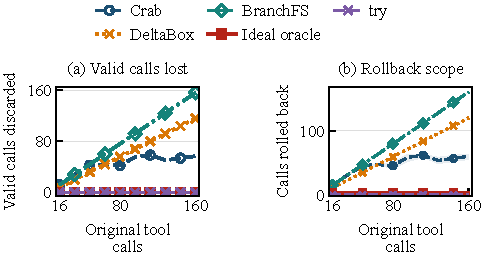
\includegraphics[width=\linewidth]{FIG-Motivation-Coarse-Waste.pdf}
  \caption{\textbf{Recovery loss versus trajectory length.}
  \small\emph{Fixed trajectories with four affected calls and exact fault
  information. (a) Independent calls discarded; (b) total calls rolled back
  as trajectory length increases. Points average ten cases; bands show
  95\% case-bootstrap intervals. \trycmd removes only one of the
  four affected calls.}}
  \label{fig:motivation-coarse-waste}
\end{figure}

Across all 400 cases, Crab, DeltaBox, and BranchFS discard 54.02\%, 56.90\%, and 100\% of valid work on average.
These losses occur with exact fault information. Even Crab,
given the exact affected turns, discards the independent calls within
those turns.

\trycmd discards no independent work but removes only 17.03\%
of affected calls on average. It clears the entire affected set in only
10 of 400 cases (2.5\%), all with no dependent calls.

To explain these losses, we next examine where independent calls occur
relative to calls affected by the error.

\textbf{Observation \#2: Calls executed after an error are not necessarily
affected by it.}
In Figure~\ref{fig:motivation-rollback-example}, the update to E occurs after
the faulty write to A but does not depend on it. The later read of A does.
Both calls execute after the error, but only the read consumes the faulty
state. Rolling back both would discard the valid update made by E.

In 390 of the 400 trajectory cases (97.5\%), returning to a checkpoint cannot
remove every affected step without also discarding valid work. Only the
remaining ten cases allow temporal rollback to remove all affected steps
and preserve all independent work.

Figure~\ref{fig:motivation-dependency}(a) varies the percentage of later calls
that depend on the faulty call, from 0\% (none) to 100\% (all), in an 80-call
execution. This sweep uses 210 fixed trajectories, ten per point, with exact
fault information. The x-axis gives the fraction of later calls affected by
the faulty call; Figure~\ref{fig:motivation-dependency}(a) reports the
minimum valid work discarded, using the deterministic token weights.
With no dependent later calls, Crab discards 18.99\%
of valid work and DeltaBox discards 74.68\%.
DeltaBox removes exactly
the affected calls only in the ten fully dependent cases, losing independent
work in the other 200 cases.

Figure~\ref{fig:motivation-dependency}(b) shows why this loss occurs.
The execution length and fault position stay fixed, so DeltaBox
always removes 60 calls. Yet the actual affected set grows from one to 60
calls as dependencies increase. At 0\%, DeltaBox discards 59 valid
calls along with the faulty call; only at 100\% are all 60 calls affected.
The Ideal oracle follows the affected set throughout. Thus, executing a
call after the error does not mean that the call depends on it.

\begin{figure}[!ht]
  \centering
  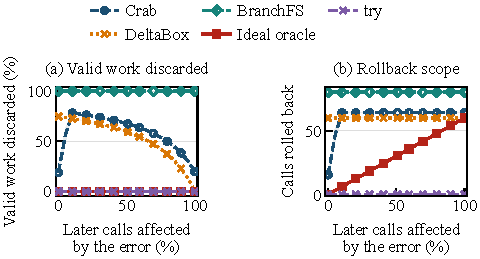
\includegraphics[width=\linewidth]{FIG-Motivation-Dependency.pdf}
  \caption{\textbf{Recovery loss versus affected-call fraction.}
  \small\emph{Fixed 80-call trajectories varying the percentage of later
  calls affected by the fault. (a) Valid work discarded; (b) total calls
  rolled back, compared with the Ideal affected set. Points average ten
  cases; bands show 95\% case-bootstrap intervals. \trycmd
  withdraws only the faulty root.}}
  \label{fig:motivation-dependency}
\end{figure}

The Ideal oracle discards no valid work throughout the sweep. The gap is
largest when many later calls are independent of the error. Selection by
dependency preserves those calls, whereas temporal rollback removes
everything after a point in time. The controlled cases establish this opportunity; the next
observation asks whether real agent executions contain the same interleaving.

\textbf{Observation \#3: Dependencies interleave with independent work
in real agent executions.}
The controlled cases show why a time boundary can include valid work. We
next check whether the same structure arises when agents autonomously solve
benchmark tasks. SWE-agent and Codex each run 300 SWE-Bench Lite~\cite{swebench}
and 241 Terminal-Bench~\cite{tbench} tasks with live LLM calls and no injected
faults. All 1,082 runs finished. We analyze 946 complete traces, including
failed attempts and traces with no recovery opportunity; the 38 partial traces and
98 invalid captures are reported separately.

Offline analysis combines file and result dependencies, recorded parents,
and opaque-context barriers. Useful calls access task files or build
artifacts, or return nonempty task observations; adapter polling, patch
retrieval, and submission are excluded. For Codex, read tracing covers the
traced processes and their descendants; failed lookups do not count as
evidence that a directory exists.
Interleaving requires useful calls $i<j<k$: $i$ changes files or returns an
observation, $k$ depends on $i$, and $j$ lies outside the dependent closure of $i$.

Figure~\ref{fig:motivation-native-opportunity} reports the recorded
dependencies for both agents and benchmarks.
Figure~\ref{fig:motivation-native-opportunity}(a) considers only file
dependencies. Figure~\ref{fig:motivation-native-opportunity}(b) considers
both file dependencies and dependencies carried through agent context,
where later calls reuse earlier tool results. It counts traces in which
independent work occurs between dependent calls. The two panels measure
different properties: (a) counts traces with file dependencies, while (b)
counts interleaving under the combined file and result graph.
Both use all complete captures as the denominator, including failed task
attempts and zero-opportunity traces. SWE and TB denote SWE-Bench Lite
and Terminal-Bench; $N$ gives the numbers of complete traces for SWE-agent
followed by Codex.


\begin{figure}[!ht]
  \centering
  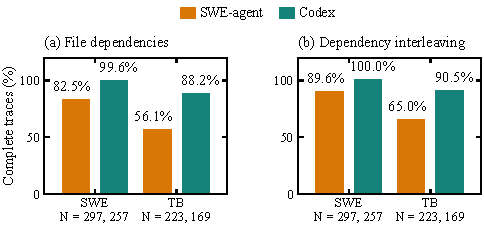
\includegraphics[width=\linewidth]{FIG-Motivation-Native-Opportunity.pdf}
  \caption{\textbf{File dependencies and interleaving in real traces.}
  \small\emph{Percentage of complete clean traces with (a) file dependencies
  and (b) dependency interleaving across files and agent context.
  SWE and TB denote
  SWE-Bench Lite and Terminal-Bench; $N$ lists trace counts for SWE-agent,
  then Codex.}}
  \label{fig:motivation-native-opportunity}
\end{figure}

File dependencies occur in 245/297 SWE-agent and 256/257 Codex SWE-Bench
traces (82.5\% and 99.6\%), and 125/223 SWE-agent and 149/169 Codex
Terminal-Bench traces (56.1\% and 88.2\%; Figure~\ref{fig:motivation-native-opportunity}(a)). Thus, the effects of a call
are reused by later calls in both benchmarks and agent systems.

Figure~\ref{fig:motivation-native-opportunity}(b) shows dependency interleaving in 266/297 SWE-agent and 257/257
Codex SWE-Bench traces (89.6\% and 100\%), and 145/223 SWE-agent and
153/169 Codex Terminal-Bench traces (65.0\% and 90.5\%). Overall,
821/946 traces (86.8\%) contain a dependent pair separated by independent
task work. If recovery withdraws file effects or an observation produced by
a call, rolling back to before that call also removes the intervening
independent work. The mismatch in Observation~\#2 is therefore common in
autonomous benchmark trajectories.

\subsection{Motivation}
\label{sec:recovery-challenges}

Together, these observations motivate recovery that follows dependencies
across both files and tool results. Given a user-specified file, the goal
is to withdraw its mutations since a reference checkpoint and their
dependent calls while preserving independent file updates and observations.

\textbf{Attempts.}
The recovery scopes examined above fall short in different ways:
1) The Crab scope clears affected turns but also discards
independent calls within them; 2) the DeltaBox and BranchFS scopes remove
affected work together with independent progress. Even with exact fault
information, these scopes incur the loss shown in
Figures~\ref{fig:motivation-coarse-waste} and~\ref{fig:motivation-dependency}.

\textbf{Insight.}
An error can spread from a file into a tool result and back into a later
file change, while independent calls occur in between. Following file
dependencies alone can therefore miss calls that reuse a returned value.
Evidence from both channels guides the selection of calls to withdraw.
Tool calls provide a practical recording unit: each call links
file accesses and mutations to a result that the agent can reuse.

\textbf{Challenges.}
Realizing this strategy raises three questions:
1) How can recovery derive and check a rollback set from a user-specified
file when its effects propagate through both file state and reused tool results?
2) How can the filesystem combine historical versions of affected
objects with current independent updates, when no checkpoint contains the
desired state?
3) How can the same rollback set update the agent context, removing
withdrawn calls and results from mixed turns while preserving independent
observations, so the next model request matches the restored filesystem?
Section~\ref{sec:design} answers these questions through rollback-set
selection, filesystem reconstruction, and agent-context alignment.
